\chapter{Comment utiliser l'application}

Cette application se nomme \textbf{Chronos}, et vous permet de configurer des alarmes en conversant avec un agent. Pour que l'agent accepte de configurer votre alarme,
vous devrez fournir une date ainsi qu'une heure lors de votre échange avec ce dernier. Si vous êtes satisfait de l'alarme que vous voulez configurer, alors vous
aurez la possibilité de le confirmer et l'agent préparera ainsi cette alarme, qui, lors de son déclenchement, sera accompagnée d'une musique liée à la météo de votre
géolocalisation. \textbf{Attention :} Pour le moment, pour qu'une alarme se déclenche, il ne faut pas tuer l'application et la laisser tourner en tâche de fond.

\section{Pré-requis}
Nous supposerons que vous posséder un smartphone avec une version d'Android supérieure à 4.2.x. Vous devez également avoir installé l'application
en suivant le manuel d'installation.\\

Dans la suite de ce manuel, vous retrouverez les icônes suivantes qui vous donneront des informations :

\begin{figure}[H]
  \centering
  
\includegraphics[width=2cm]{images/hand.png}
  \caption{Cette icône vous indique soit un endroit ou cliquer à l'écran de votre smartphone, soit attire votre attention sur un détail en particulier.}
\end{figure}

\begin{figure}[H]
  \centering
  
\includegraphics[width=2cm]{images/voice.png}
  \caption{Cette icône vous indique que vous devez parler dans le microphone de votre smartphone.}
\end{figure}

\section{Ouverture de l'application}

Vous pouvez ouvrir l'application en cliquant dessus comme suit :

\begin{figure}[H]
  \centering
  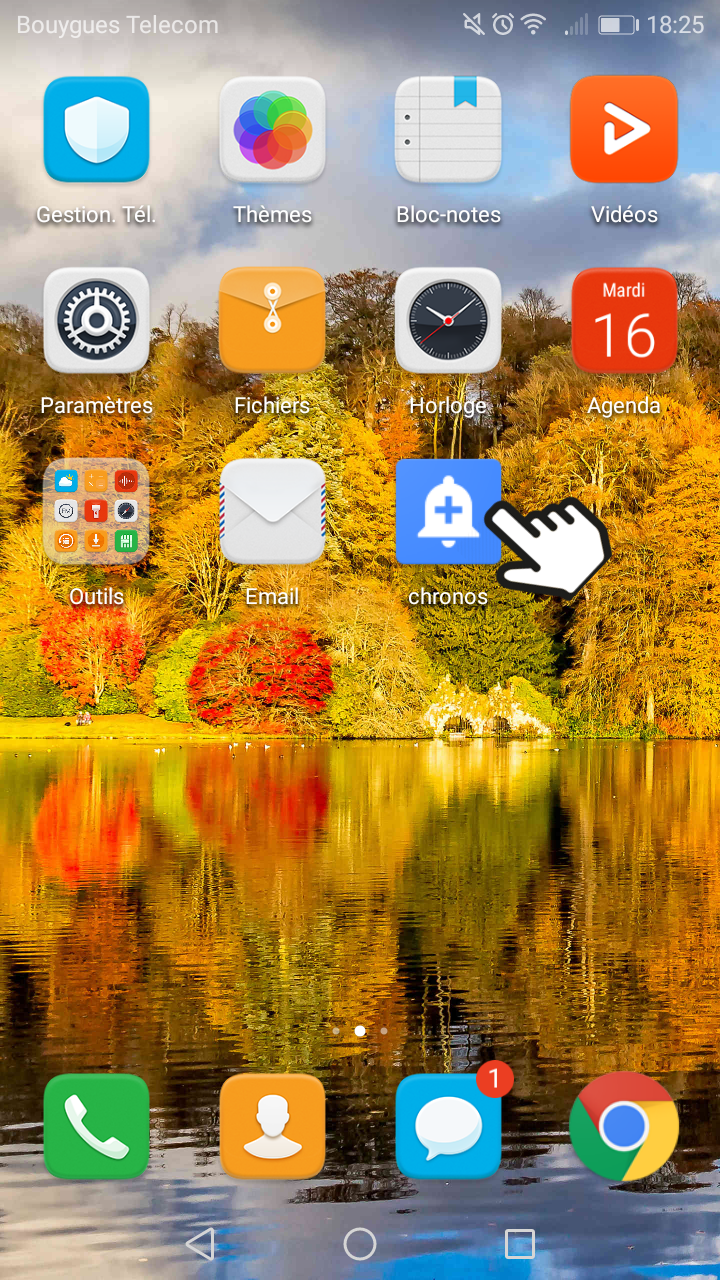
\includegraphics[width=6cm]{images/A.png}
  \caption{Ouverture de l'application}
\end{figure}

\begin{figure}[H]
  \centering
  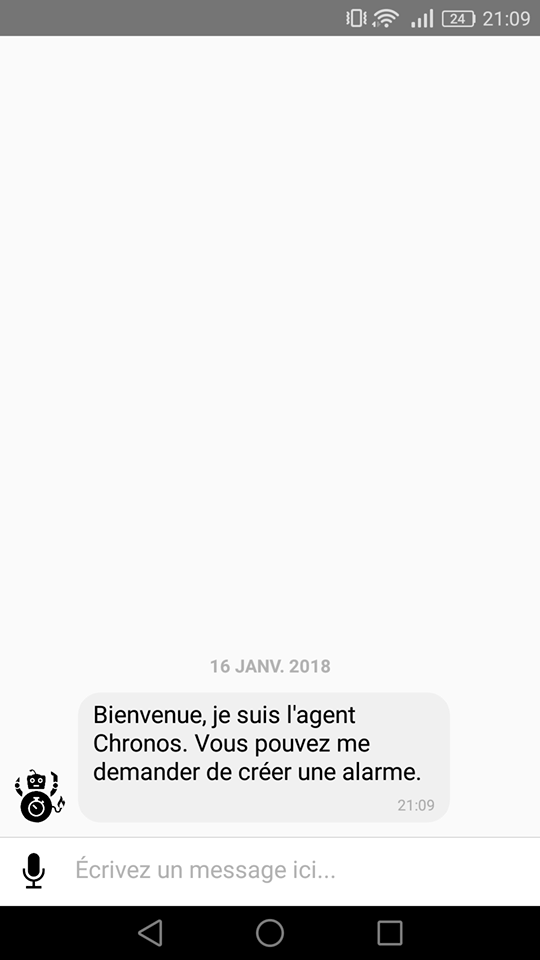
\includegraphics[width=6cm]{images/B1.png}
  \caption{Ecran principal}
\end{figure}

Une fois l'application ouverte, vous tombez sur l'écran suivant. Vous pouvez communiquer avec l'agent via le microphone en appuyant une fois sur l'icône de micro
ou directement en entrant le texte dans le champ texte se situant à coté de l'icône de micro. Vous n'êtes pas obligé de donner à l'agent l'ensemble des données
dont il a besoin pour configurer votre alarme - en effet vous pouvez très bien y aller étape par étape comme nous allons le voir. Vous pouvez commencer par cliquer
une fois sur l'icône micro et dire que vous désirez mettre une alarme :

\begin{figure}[H]
  \centering
  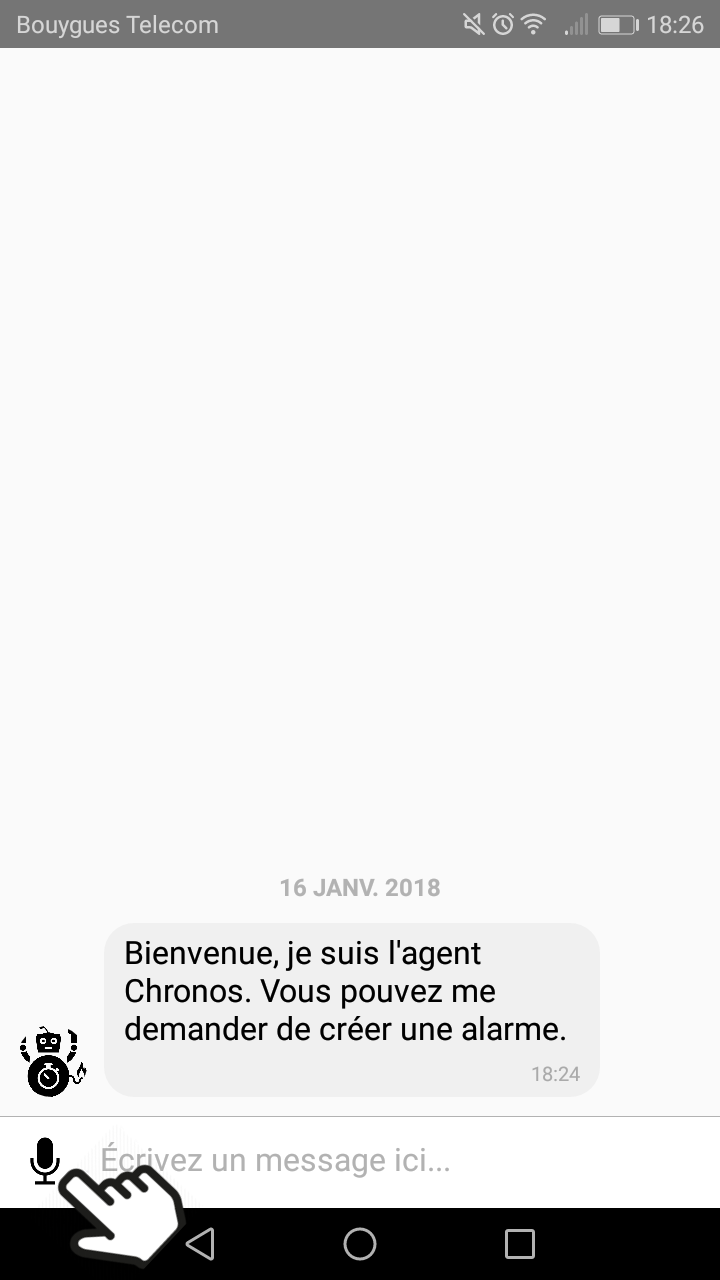
\includegraphics[width=6cm]{images/B.png}
  \caption{Cliquer sur l'icône micro}
\end{figure}

\begin{figure}[H]
  \centering
  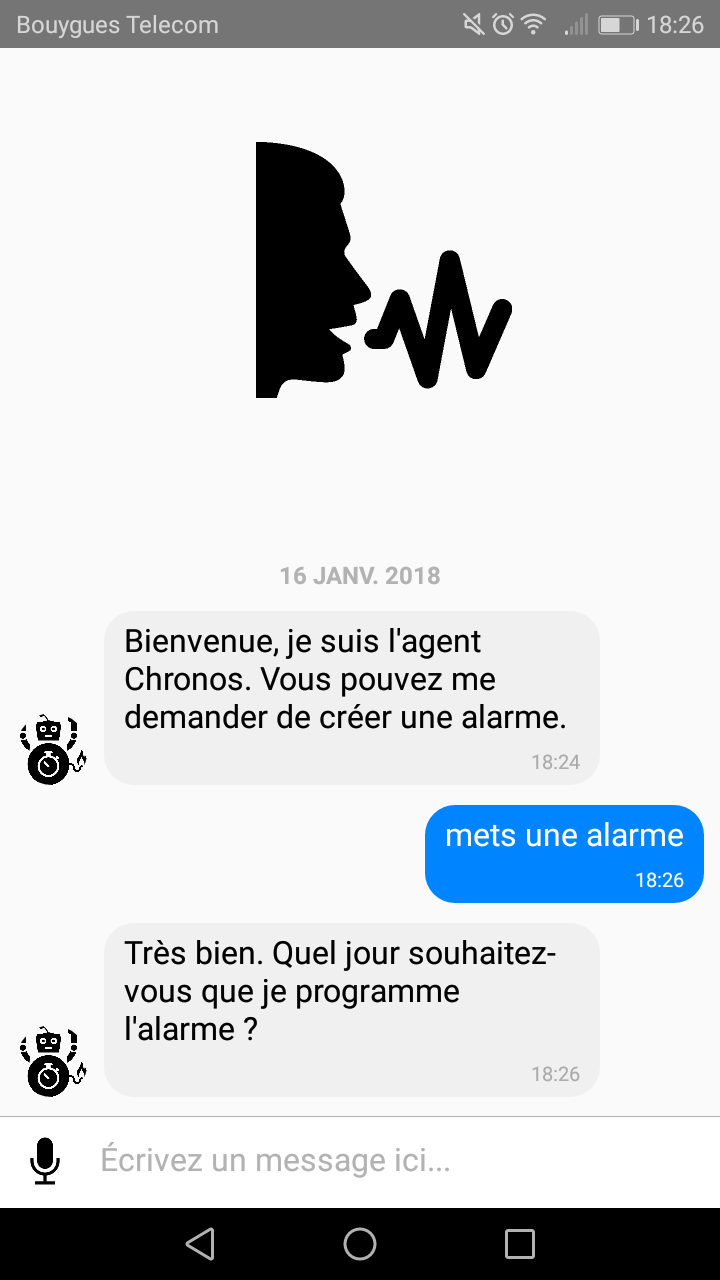
\includegraphics[width=6cm]{images/C.png}
  \caption{Demander la programmation d'une alarme avec la voix}
\end{figure}

L'application détectera automatiquement que vous avez cessé de parler, vous n'avez donc pas besoin de ré-appuyer sur l'icône micro pour signaler la fin de votre phrase.
Ensuite, vous pouvez indiquer la date à laquelle déclencher l'alarme en cliquant de nouveau sur l'icône micro :

\begin{figure}[H]
  \centering
  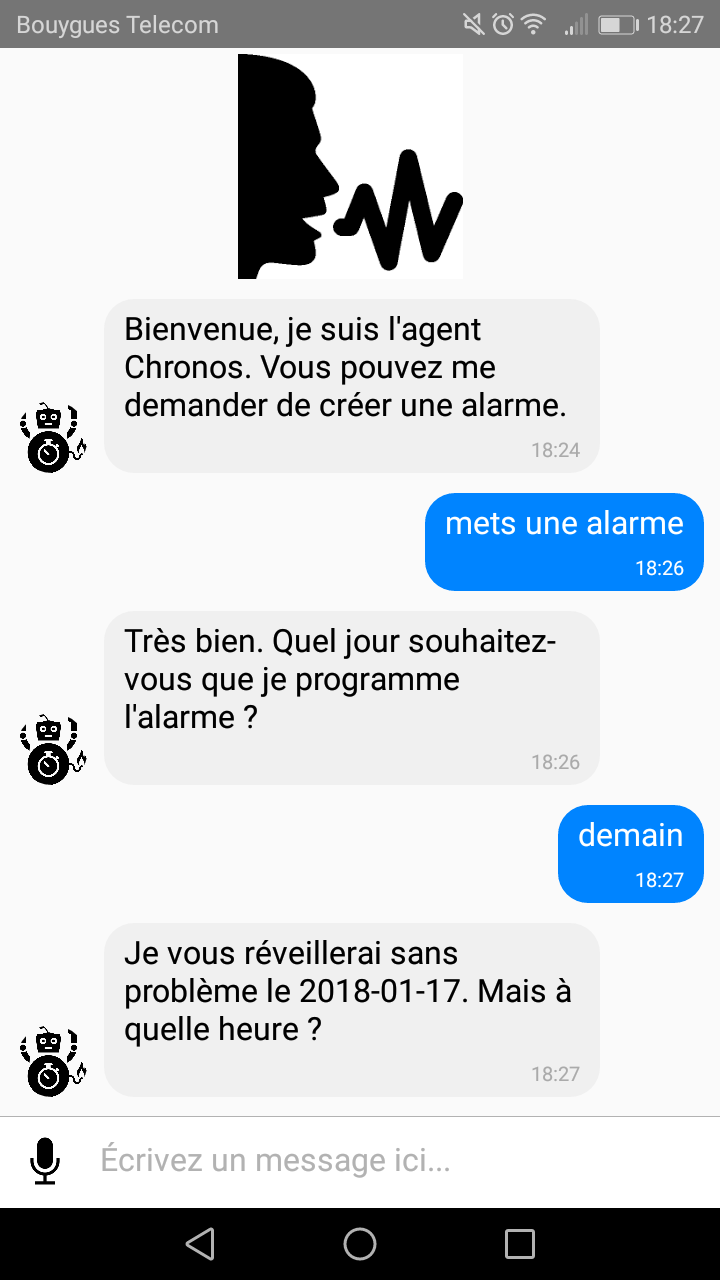
\includegraphics[width=6cm]{images/D.png}
  \caption{Indiquer la date avec la voix}
\end{figure}

Puis pour finir en lui indiquant l'heure à laquelle déclencher l'alarme. S'il a bien reconnu votre intention, l'agent vous demandera ensuite une confirmation comme suit :

\begin{figure}[H]
  \centering
  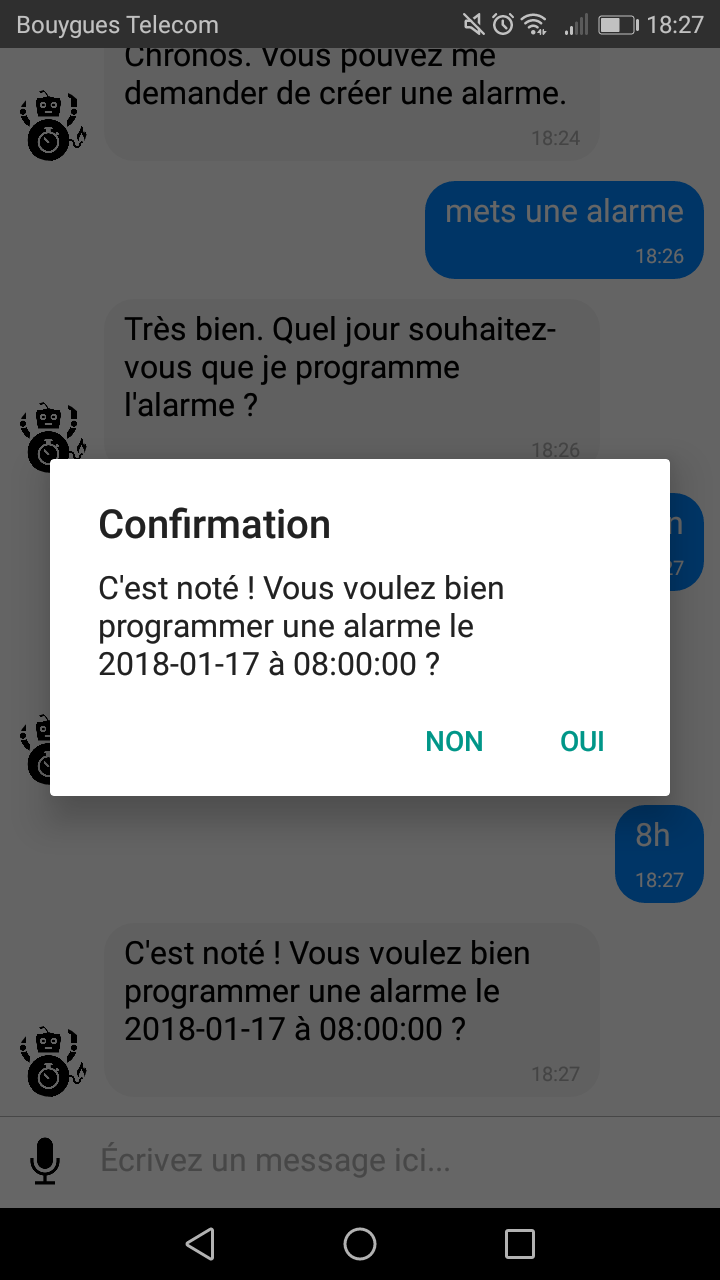
\includegraphics[width=6cm]{images/E.png}
  \caption{Indiquer l'heure et confirmer ou non}
\end{figure}

Vous auriez très bien pu converser avec l'agent via l'entrée textuelle :

\begin{figure}[H]
  \centering
  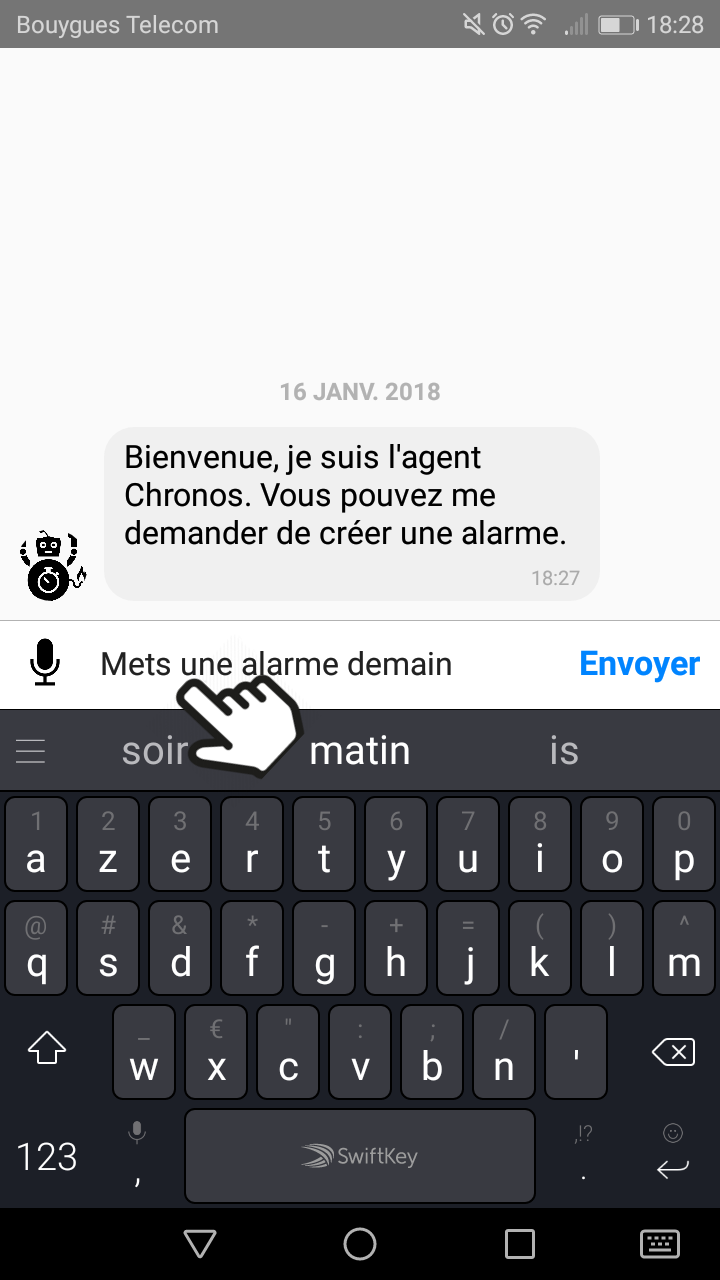
\includegraphics[width=6cm]{images/F.png}
  \caption{Demande de programmation d'une alarme via texte}
\end{figure}

Si vous avez confirmé la programmation de l'alarme, l'agent vous indiquera la météo prévisionnelle associée à votre alarme. Comme le montre la
figure suivante, vous pouvez également programmer l'alarme en unse seule phrase si celle-ci est complète :

\begin{figure}[H]
  \centering
  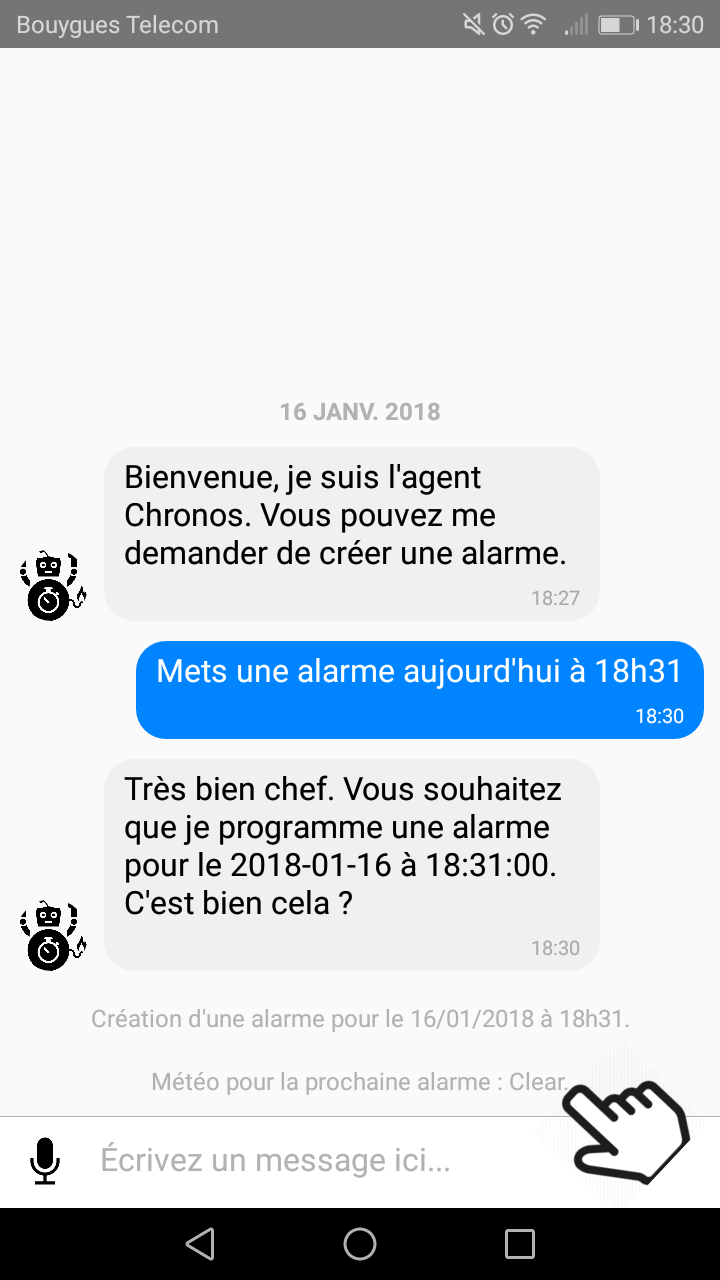
\includegraphics[width=6cm]{images/G.png}
  \caption{Météo prévisionnelle de l'alarme}
\end{figure}

Lorsque qu'une alarme se déclenchera, vous recevrez une notification accompagnée de la musique associée à la météo liée à votre localisation :

\begin{figure}[H]
  \centering
  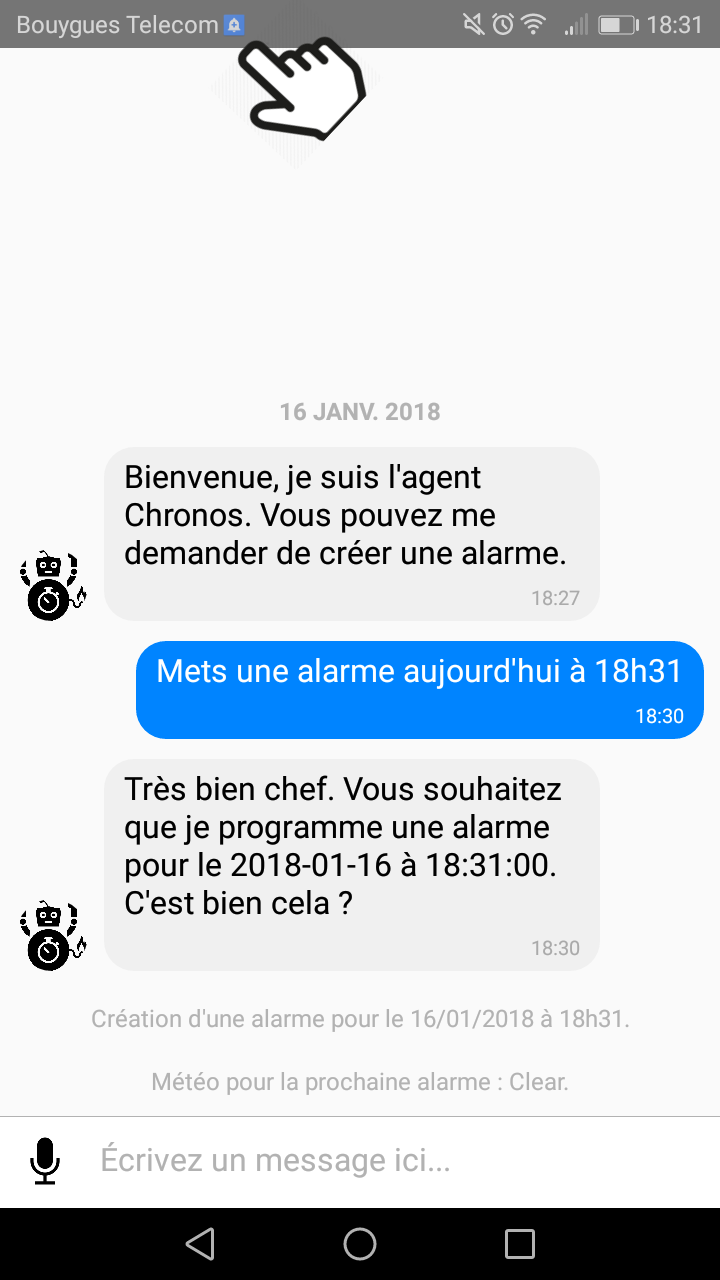
\includegraphics[width=6cm]{images/H.png}
  \caption{Déclenchement d'une alarme : notification}
\end{figure}

Petit bonus, l'agent reconnaîtra quelques phrases supplémentaires non liées à la fonctionnalité prévue pour l'application, à vous de les découvrir ;)

\begin{figure}[H]
  \centering
  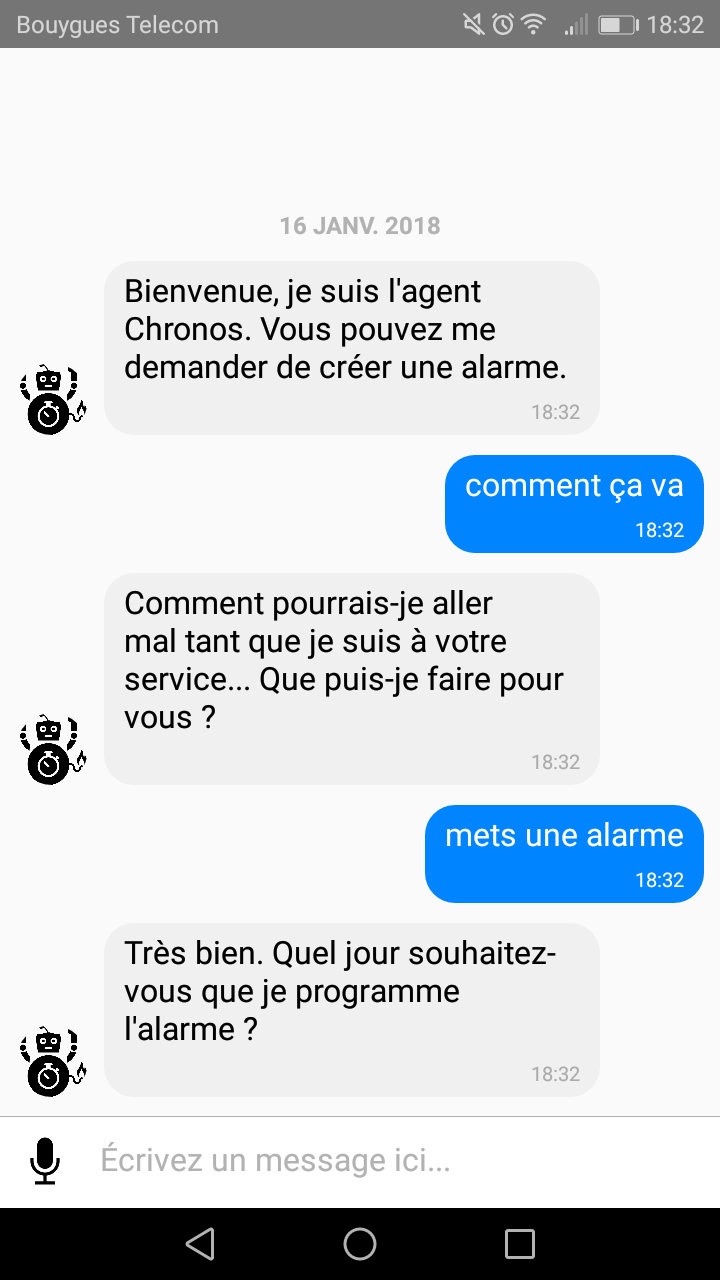
\includegraphics[width=6cm]{images/J.png}
  \caption{Petite conversation bonus}
\end{figure}
